\documentclass[11pt]{article}
\usepackage{fontspec}
\usepackage{amsmath}
\usepackage{amsfonts}
\usepackage{amssymb}
\usepackage[letterpaper,margin=1in]{geometry}
\usepackage[hidelinks]{hyperref}
\usepackage[nameinlink]{cleveref}
\usepackage{tikz}
\usepackage{pgfplots}
\usepackage{fancyhdr}
\usepackage{cancel}

\title{Calculus Q3 Proofs}
\author{Adam Zhang}

\crefname{proof}{Proof}{Proofs}
\crefalias{enumi}{proof}

\setlength\parindent{0pt}

\begin{document}
\pagestyle{fancy}
\fancyhead[L]{AET Multivariable Calculus \\ \textbf{Quarter 3 Proofs}}
\fancyhead[R]{Adam Zhang \\}

\begin{center}
  \emph{On my honor, I will not accept nor provide any unauthorized aid on this assignment.}
\end{center}

\section*{Proofs}
\begin{enumerate}
\item Assume that all the given functions have continuous second-order partial
  derivatives. Show that any function of the form \(z = f(x + at) + g(x - at) \)
  is a solution of the wave equation \(\frac{\partial^2 z}{\partial t^2} = a^2
  \frac{\partial^2 z}{\partial x^2}\) (\textit{Hint}: Let \( u = x + at \), \( v
  = x - at \)).

  \begin{align*}
    z &= f(u) + g(v) \\
    \frac{\partial z}{\partial t}
      &= f'(u) \frac{\partial u}{\partial t} + g'(v) \frac{\partial
        v}{\partial t} \\
      &= a f'(u) -a g'(v) \\
    \frac{\partial^2 z}{\partial t^2}
      &= a f''(u) \frac{\partial u}{\partial t} - a g''(v) \frac{\partial
        v}{\partial t} \\
      &= a^2 f''(u) + a^2 g''(v) \\
      &= a^2 (f''(u) + g''(v)) \\
    \frac{\partial z}{\partial x}
    &= f'(u) \frac{\partial u}{\partial x} + g'(v) \frac{\partial v}{\partial x}
    \\
      &= f'(u) + g'(v) \\
    \frac{\partial^2 z}{\partial x^2}
    &= f''(u) \frac{\partial u}{\partial x} + g''(v) \frac{\partial v}{\partial x} \\
    &= f''(u) + g''(v) \\
  \end{align*}

\item Suppose that directional derivatives of \(f(x,y)\) are known at a point in two nonparallel directions given by unit vectors \(\vec{u} = \langle a, b \rangle\) and \(\vec{v} = \langle c, d \rangle\). Let the directional derivatives be defined as \(D_{u} f\) and \(D_{v} f\). Is it possible to find \( \nabla f \) at this point? If so, find \( \nabla f \) in terms of \( D_{u} f \), \( D_{v} f \), and the unit vectors \(\vec{u} = \langle a, b \rangle\) and \(\vec{v} = \langle c, d \rangle\).

  \begin{align*}
    D_uf = \nabla f \cdot \vec{u} &\qquad D_vf = \nabla f \cdot \vec{v} \\
    D_uf = a f_x + b f_y &\qquad D_vf = c f_x + d f_y \\
    \begin{bmatrix}
      a & b \\
      c & d \\
    \end{bmatrix}
    \begin{bmatrix}
      f_x \\ f_y
    \end{bmatrix}
    &=
      \begin{bmatrix}
        D_uf \\ D_v f
      \end{bmatrix} \\
    \nabla f
    &=
      \frac{1}{ad - bc}
      \begin{bmatrix}
        d & -b \\
        -c & a \\
      \end{bmatrix}
      \begin{bmatrix}
        D_uf \\ D_v f
      \end{bmatrix} \\
    &= \left< \frac{d D_uf - b D_vf}{ad - bc}, \frac{a D_vf - c D_uf}{ad - bc} \right>
  \end{align*}

\item Are there any points on the hyperboloid \(x^2 - y^2 - z^2 = 1\) where
  the tangent plane is parallel to the plane \(z = x + y\)? If yes, find
  the point(s). If no, clearly explain why.

  \begin{align*}
    \text{Plane: }& x + y - z = 0 \\
                  &\vec{N} = \left< 1, 1, -1 \right> \\
    \text{Hyperboloid: }& f(x, y, z) = x^2 - y^2 - z^2 \\
                  &\nabla f = \left< 2x, -2y, -2z \right> \\
    \lambda\vec{N} &= \nabla f
                     \begin{cases}
                       2x &= \lambda \\
                       -2y &= \lambda \\
                       -2z &= \lambda
                     \end{cases} \\
    2x &= -2y \\
    y &= -x \\
    -2y &= -2z \\
    y &= z = -x \\
    x^2 - (-x)^2 - (-x)^2 &= 1 \\
    x^2 &\neq -1
  \end{align*}

\item Use Lagrange Multipliers to prove that the triangle with maximum area that
  has a given perimeter \(p\) is equilateral.

  \textit{Hint}: Use Heron's formula for the area:
  \(A = \sqrt{s(s - x)(s - y)(s - z)}\) where \(s = \frac{p}{2}\) and
  \(x, y, z\) are the lengths of the sides.

  \begin{align*}
    A &= \sqrt{s(s - x)(s - y)(s - z)} \\
    A^2 &= s(s - x)(s - y)(s - z) \\
    f(x, y, z) &= s(s - x)(s - y)(s - z) \\
    \nabla f &= \left< -s(s - y)(s - z), -s(s - x)(s - z), -s(s - x)(s - y) \right> \\
    g(x, y, z) &= x + y + z = 2s \\
    \nabla g &= \left< 1, 1, 1 \right> \\
    \nabla f &= \lambda\nabla g
               \begin{cases}
                 -s(s - y)(s - z) &= 1 \cdot \lambda \\
                 -s(s - x)(s - z) &= 1 \cdot \lambda \\
                 -s(s - x)(s - y) &= 1 \cdot \lambda \\
               \end{cases} \\
    -s(s - y)(s - z) &= -s(s - x)(s - z) \\
    s - y &= s - x \\
    y &= x \\
    -s(s - x)(s - z) &= -s(s - x)(s - y) \\
    s - z &= s - y \\
    z &= y = x \\
  \end{align*}

\item Prove that \(\nabla (FG) = F \nabla G + G \nabla F\) where \(F\) and
  \(G\) are differentiable scalar functions of \(x, y\) and \(z\).

  Let \(H(x, y, z) = F(x, y, z) G(x, y, z)\).

  \begin{align*}
    \nabla H &= \left< H_x, H_y, H_z \right> \\
             &= \left< FG_x + GF_x, FG_y + GF_y, FG_z + GF_z \right> \\
             &= \left< FG_x, FG_y, FG_z \right> + \left< GF_x, GF_y, GF_z \right> \\
             &= F \nabla G + G \nabla F
  \end{align*}

\item If \(f(x,y)\) is continuous on \([a,b] \times [c,d]\) and
  \(g(x,y) = \int_0^x \int_0^y f(s,t) \, \mathrm{d}t \, \mathrm{d}s\) for
  \(a < x < b, c < y < d\), show that \(g_{xy} = g_{yx} = f(x,y)\).

  By Clairaut's theorem, \(g_{xy} = g_{yx}\). By the Fundamental Theorem of
  Calculus, \(\frac{\mathrm{d}}{\mathrm{d}x} \int_0^x f(a) \mathrm{d}a = f(a)\).

  \begin{align*}
    g_{xy} &= \frac{\partial}{\partial y} \frac{\partial}{\partial x} \int_0^x \int_0^y f(s,t) \, \mathrm{d}t \, \mathrm{d}s \\
           &= \frac{\partial}{\partial y} \int_0^y f(x, t) \, \mathrm{d}t \\
           &= f(x, y) \\
  \end{align*}

\item Prove Property 10 from page 1059 in Section 15.2.
  \begin{quote}
    If \(m \leq f(x,y) \leq M\) for all \((x,y)\) in \(D\), then
    \(m \cdot A(D) \leq \iint_D f(x,y) \, \mathrm{d}A \leq M \cdot A(D)\).
  \end{quote}

  Consider the constant functions \(g(x, y) = m\) and \(h(x, y) = M\). Given
  that a double integral is equivalent to signed volume under a surface in
  \(\mathbb{R}^3\), the integral of these functions over a domain \(D\) is
  equivalent to the signed volume of the rectangular prism formed by a base with
  area \(A(D)\) and height \(m\)/\(M\)\footnote{This proof is left as an
    exercise for the reader.}. Given
  \(\forall (x, y) \in D : m \leq f(x, y) \leq M\), the signed volume under the
  surface of \(f\) on \(D\) must be between \(m \cdot A(D)\) and
  \(M \cdot A(D)\) (the signed volume of the previously defined rectangular
  prisms).
\end{enumerate}

\section*{True or False}
Prove that the given statement is true or provide a counterexample to show that it is false.

\begin{enumerate}
  \setcounter{enumi}{7}

\item If \(f\) has a local minimum at \((a,b)\) and \(f\) is differentiable at
  \((a,b)\), then \(\nabla f (a,b) = \vec{0}\).

  Consider the case where \(\nabla f(a, b) \neq \vec{0}\). In this case,
  \(\nabla f\) indicates the direction of greatest change of \(f\) at
  \((a, b)\). Thus, moving in the direction of \(\nabla f\) would increase the
  value of \(f\); consequently, moving in the direction of \(-\nabla f\) would
  decrease the value of \(f\), meaning that \(f(a, b)\) cannot be a minimum.

\item If \(f(x,y)\) has two local maxima, then \(f\) must have a local minimum.

  Consider the function \(f(x, y) = x^2 - x^4 - y^2\). Solve possible
  critical points:

  \begin{align*}
    \nabla f(x, y) = &\left< 2x - 4x^3, -2y \right> \\
    \vec{0} = \left< 2x - 4x^3, -2y \right>
    &\begin{cases}
      2x - 4x^3 &= 0 \\
      -2y &= 0 \\
    \end{cases} \\
    x(2 - 4x^2) &= 0 \\
    x(\sqrt{2} + 2x)(\sqrt{2} - 2x) &= 0 \\
    x &= \left\{ 0, \pm \frac{\sqrt{2}}{2} \right\} \\
    y &= 0
  \end{align*}

  Thus, \(f\) has local maxima at
  \((\pm \frac{1}{\sqrt{2}}, 0, f(\frac{1}{\sqrt{2}}, 0))\). However, \((0, 0)\)
  is neither a maximum nor minimum point (rather, it's a saddle point); thus,
  \(f(x, y)\) has no minima\footnote{This is trivially verifiable by considering
    that, since all critical points lie on the plane \(y = 0\), any extrema must
    also be extrema on the \(x\) portion of \(f\). The maxima and lack of minima
    for \(f(x) = x^2 - x^4\) is trivially verifiable using single-variable
    calculus.}.
\end{enumerate}

\textit{For problems \#10--12, if the answer is false, your explanation must include what the correct integral should be.}

\begin{enumerate}
  \setcounter{enumi}{9}
  
\item
  \(\int_{-\frac{1}{2}}^{2} \int_{y^2}^{\frac{3}{2}y+1} x^2 \sin(x-y)
  \,\mathrm{d}x\,\mathrm{d}y = \int_0^4 \int_{\frac{2}{3}(x-1)}^{\sqrt{x}} x^2
  \sin(x-y) \, \mathrm{d}y \, \mathrm{d}x\) \label{proof:10}

  \begin{figure}[h]
    \centering
    \caption{Plot of Integration Regions for \cref{proof:10}}
    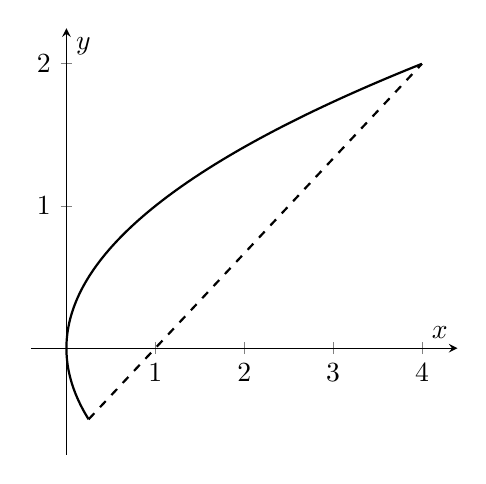
\begin{tikzpicture}
      \begin{axis}[
        width=7cm,
        height=7cm,
        axis lines=middle,
        xlabel={$x$}, ylabel={$y$},
        xtick={-1,0,1,2,3,4},
        ytick={-1,0,1,2,3},
        enlargelimits=true,
        domain=-0.5:2,
        samples=100,
        ]
        \addplot[black, dashed, thick] ({(3/2)*x+1}, x) node[right] {};
        \addplot[black, thick] ({x^2}, x) node[right] {};
      \end{axis}
    \end{tikzpicture}
    \hspace{1cm}
    \begin{tikzpicture}
      \begin{axis}[
        width=7cm,
        height=7cm,
        axis lines=middle,
        xlabel={$x$}, ylabel={$y$},
        xtick={0,1,2,3,4},
        ytick={-1,0,1,2},
        enlargelimits=true,
        domain=0:4,
        samples=100,
        ]
        \addplot[black, dashed, thick] {(2/3)*(x-1)} node[right] {};
        \addplot[black, thick] {sqrt(x)} node[right] {};
      \end{axis}
    \end{tikzpicture}
  \end{figure}
  
\item
  \(\int_0^{\pi/4} \int_{\sin x}^{\cos x} \sqrt{x + y^2} \, \mathrm{d}y\,
  \mathrm{d}x = \int_0^1 \int_{\arcsin y}^{\arccos y} \sqrt{x + y^2} \,
  \mathrm{d}x\, \mathrm{d}y\)

\item
  \(\int_{-1}^{1} \int_{0}^{1} e^{x^2 + y^2} \sin y \, \mathrm{d}x\,
  \mathrm{d}y= 0\)

  Consider \(x^2\) and \(y^2\), which are both even functions. Thus, both
  \(x^2 + y^2\) and \(e^{x^2 + y^2}\) are even
  functions\footnote{\label{fn:trivial} This trivial proof is left as an
    exercise for the reader.}. Consider \(\sin(y)\), which is an odd
  function\footnotemark[\value{footnote}]. Thus, the function
  \(e^{x^2 + y^2} \sin y\) is an odd function along the
  \(y\)-axis\footnotemark[\value{footnote}]. Therefore, the integral from
  \(y = -1\) to \(y = 1\) is zero.
\end{enumerate}

\end{document}
